\documentclass[10pt,landscape]{article}
\usepackage{multicol}
\usepackage{calc}
\usepackage{ifthen}
\usepackage[landscape]{geometry}
\usepackage{amsmath,amsthm,amsfonts,amssymb}
\usepackage{color,graphicx,overpic}
\usepackage{bm}
\usepackage{hyperref}



% This sets page margins to .5 inch if using letter paper, and to 1cm
% if using A4 paper. (This probably isn't strictly necessary.)
% If using another size paper, use default 1cm margins.
\ifthenelse{\lengthtest { \paperwidth = 11in}}
    { \geometry{top=1cm,left=1cm,right=1cm,bottom=1cm} }
    {\ifthenelse{ \lengthtest{ \paperwidth = 297mm}}
        {\geometry{top=1cm,left=1cm,right=1cm,bottom=1cm} }
        {\geometry{top=1cm,left=1cm,right=1cm,bottom=1cm} }
    }

% Turn off header and footer
\pagestyle{empty}

% Redefine section commands to use less space
\makeatletter
\renewcommand{\section}{\@startsection{section}{1}{0mm}%
                                {-1ex plus -.5ex minus -.2ex}%
                                {0.5ex plus .2ex}%x
                                {\normalfont\large\bfseries}}
\renewcommand{\subsection}{\@startsection{subsection}{2}{0mm}%
                                {-1explus -.5ex minus -.2ex}%
                                {0.5ex plus .2ex}%
                                {\normalfont\normalsize\bfseries}}
\renewcommand{\subsubsection}{\@startsection{subsubsection}{3}{0mm}%
                                {-1ex plus -.5ex minus -.2ex}%
                                {1ex plus .2ex}%
                                {\normalfont\small\bfseries}}
\makeatother
\newenvironment{lmat}
{\left|\begin{smallmatrix}}
	{\end{smallmatrix}\right|}

\newcommand{\deriv}[1]{\frac{\mathrm{d}}{\mathrm{d}#1} }

% For partial derivatives
\newcommand{\pderiv}[2]{\frac{\partial #1}{\partial #2}}

% Integral dx
\newcommand{\dx}{\mathrm{d}x}
\newcommand{\cd}{\overset{d}{\to}}
\newcommand{\cp}{\overset{p}{\to}}
\newcommand{\B}{\beta}
\newcommand{\e}{\epsilon}
\newcommand{\limn}{\lim_{n\to \infty}}
\newcommand{\lm}{\lambda}
\newcommand{\sg}{\sigma}
\newcommand{\hb}{\hat{\beta}}
\newcommand{\sumn}{\sum_{i=1}^{n}}
\newcommand{\hth}{\hat{\theta}}
\newcommand{\lra}{\Leftrightarrow}
\newcommand{\prodn}{\prod_{i=1}^{n}}
\newcommand{\dll}[1]{\dfrac{\partial\ell}{\partial{#1}}}
\newcommand{\mle}{\hat{\theta}_{MLE}}
\newcommand{\mm}{\hat{\theta}_{MM}}
\newcommand{\sumx}{\sum_{i=1}^{n}x_i}
\newcommand{\ta}{\theta}
\newcommand{\qe}{ \ ?\ }
\newcommand{\dt}{\pderiv{}{\ta}}
\newcommand{\dtt}{\pderiv{^2}{\ta^2}}
\newcommand{\lt}[1]{\log(f(#1|\ta))}
\newcommand{\lx}{\lambda(x)}
\newcommand{\dtau}{\left(\dfrac{d\tau(\ta)}{d \ta}\right)^2}
\newcommand{\samp}{X_1,\dots,X_n \sim}
\newcommand{\ra}{\Rightarrow}
\newcommand{\xxx}{X(X^{\prime}X)^{-1}X^{\prime}}
\newcommand{\xx}{(X^{\prime}X)^{-1}}
\newcommand{\m}{C\xx C^{\prime}}
\newcommand{\p}{\prime}
\newcommand{\hy}{\hat{y}}
\newcommand{\st}{\sg^2}
\newcommand{\sh}{\hat{\sg^2}}
\newcommand{\eh}{\hat{\epsilon}}
\allowdisplaybreaks
% Define BibTeX command
\def\BibTeX{{\rm B\kern-.05em{\sc i\kern-.025em b}\kern-.08em
    T\kern-.1667em\lower.7ex\hbox{E}\kern-.125emX}}

% Don't print section numbers
\setcounter{secnumdepth}{0}


\setlength{\parindent}{0pt}
\setlength{\parskip}{0pt plus 0.5ex}

%My Environments
\newtheorem{example}[section]{Example}
% -----------------------------------------------------------------------

\begin{document}

\raggedright
\footnotesize
\begin{multicols*}{4}
\setlength{\premulticols}{1pt}
\setlength{\postmulticols}{1pt}
\setlength{\multicolsep}{1pt}
\setlength{\columnsep}{2pt}

% multicol parameters
% These lengths are set only within the two main columns
\setlength{\columnseprule}{.25pt}
\setlength{\premulticols}{.25pt}
\setlength{\postmulticols}{.25pt}
\setlength{\multicolsep}{.25pt}
\setlength{\columnsep}{.25pt}


Orthogonal Matrix $\ra$ square mat w/ $A^{\prime}=A^{-1}$\\
If sym mat $\ra  \exists$ orth mat $V$ st $A=V\Lambda V^{\prime}$\\
$E(AY+B)=AE(Y)+b=A\mu+b$\\
$Cov(AY+b)=ACov(Y)A^{\prime}=A\Sigma A^{\prime}$\\
$Z^2=\chi^2(1)$ If $Z_1,\dots,Z_n$ ind:\\
$W=\sum Z_i^2\sim \chi^2(n)$\\
$\ra \mu=n \sg^2=2n$\\
$Z/\sqrt{W/n}\sim T(n)$ symmetric about 0\\
$X_1\sim \chi^2(n_1)\perp X_2\sim \chi^2(n_2)$:\\
$(X_1/n_1)/(X_2/n_2)\sim F(n_1,n_2)$\\
$T\sim T(v) \quad T^2\sim F(1,v)$, F is asymmetric, +\\
$(X_{n\times p})^{'}(X_{n \times p})\hb=(X_{n\times p})^{'}y_{n\times 1}$ \\
$(AB)^{'}=B^{'}A^{'}$\quad
$A^{-1}A=AA^{-1}=I$\\
$(AB)^{-1}=B^{-1}A^{-1}$\quad
$(A^{'})^{-1}=(A^{-1})^{'}$\\
$|A^{-1}|=\dfrac{1}{|A|}$\quad
$\dfrac{1}{|A|}
\begin{lmat}
a_{22}&-a_{12}\\
-a_{21}& a_{11}
\end{lmat}$\\
det(inv)=inv(det)\quad
evector $Ax=\lm x$\quad
e val=$\lm$\\
char eqn $(|A-\lm I|=0)
=det\begin{lmat}
a_{11}-\lm & a_{12}\\
a_{21} & a_{22}-\lm
\end{lmat}$\\
full rank $\lra$ no $\lm=0$\quad
det=0  $\lra$ $\geq 1$ $\lm=0$\\
X full rank for $\hb$ unique\\
E(rand mat)=mat of E\\
$Cov(Y)=E[(Y-\mu)(Y-\mu)^{'}]=\bm{\Sigma}$\\
$\begin{lmat}
\sigma_{11}&\sigma_{12}&\cdots& \sg_{1n}\\
\sg_{21}& \vdots & \vdots & \vdots\\
\vdots & \vdots & \vdots & \vdots\\
\sg_{n1} &\cdots & \cdots& \sg_{nn} 
\end{lmat}$\\
$\sg_{ij}=Cov(Y_i,Y_j)=E[(Y_i-\mu_i)(Y_j-\mu_j)^{'}]$\\
1) \textbf{lin trans} of mvn yields  mvn.\\
If $X\sim N_n(\mu,\Sigma)$ and $Y=AX+b$\\
with $A_{r\times n}$  matrix of constants and $\bm{b}_{r \times 1}$ vector of constants. Then $Y\sim N_r(A\mu+b,A\Sigma A^{'})$\\
2) \textbf{lin combin} of ind mvns is mvn\\
$X_1,\dots,X_k$ iid $X_i\sim N_n(\mu_i,\Sigma_i)$\\
Let $Y=a_1X_1+\dots+a_kX_k$\\
Then $Y\sim N(\mu^*,\Sigma^*)$ where $\mu^{*}=\sum_{i=1}^{k}a_i\mu_i$ and $\Sigma^*=\sum_{i=1}^{k}a_i^2\Sigma_i$\\
3) \textbf{Marginals} of mvn are mvn\\
If $X\sim N_n(\mu,\Sigma)$\\
Partition:
$X={X_1 \choose X_2}$ where $X_1$ is $r\times 1$ and $X_2$ is $(n-r)\times 1$\\
$\mu={\mu_1\choose \mu_2}$ where $\mu_1$ is $r\times 1$ and $\mu_2$ is $(n-r)\times 1$\\
$\Sigma=
\begin{lmat}
\Sigma_{11}&\Sigma_{12}\\
\Sigma_{21}&\Sigma_{22}
\end{lmat}$\\
where $\Sigma_{11}$ is $r\times r$, $\Sigma_{21}$ is $(n-r)\times r$ and $\Sigma_{22}$ is $(n-r)\times (n-r)$\\
Marginals:
$X_1\sim N_r(\mu_1,\Sigma_{11})$\\ 
$X_2\sim N_{(n-r)}(\mu_2,\Sigma_{22})$\\
4) \textbf{Conditionals} of mvn are mvn.\\
Suppose $X\sim N_n(\mu,\Sigma)$\\
Partition same way\\
$X_1|X_2=x_2\sim N_r(\mu_1+\Sigma_{12}\Sigma_{22}^{-1}(x_2-\mu_2),\Sigma^*)$\\
where $\Sigma^*=\Sigma_{11}-\Sigma_{12}\Sigma_{22}^{-1}\Sigma_{21}$\\


\textbf{Topic 3, 4}
$y=X\B+\epsilon$ \quad
$\hb=(X^{'}X)^{-1}X^{'}y$\\
$\hat{y}=X\hb=Hy$\quad $H=X(X^{'}X)^{-1}X^{'}$\\
$M=C(X^{'}X)^{-1}C^{'}$\\
$\hat{\epsilon}=y-\hat{y}=y-Hy=(1-Hy)$\\
$\hth=C\hb$ \quad $\hat{Var}(\hth)=\hat{\sg^2}(C(X^{'}X)^{-1}C^{'})$\\
$\hat{Var}(\hb)=\hat{\sg^2}(X^{'}X)^{-1}$ \\
$SSH=(\hth-\theta_0)^{'}M^{-1}(\hth-\theta_0)$\\
$SSE=(y-\hat{y})^{'}(y-\hat{y})=y^{'}[I-H]y=\epsilon^{\prime}\epsilon$\\
Use MSE for $\hat{\sg^2}$, use diag\quad $df_{total}=n-1$\\
$se=\sqrt{\hat{Var}}$\quad
$MS*=SS*/DF*$\\
t-value$=\hb/se$\quad
p-value$=F(df_{model},df_{error})$\\
95\% CI  $\hth\pm 1.96\sqrt{MSE(M)}$\\
95\% PI $\hat{y_h}\pm t(\alpha/2,n-r)se(\hat{y_h})$\\
$F_{obs}=\dfrac{(\hth-\theta_0)^{'}M^{-1}(\hth-\theta_0)/a}{\hat{\sg^2}}$ $a=rank(C)$\\
$F_{obs}(1,n-r)=tval^2(n-r)$\\
One-sided t-Test (only for scalar hypothesis)\\
$H_A:\ta<\ta_0$ Uses $\alpha$ $H_A:\ta>\ta_0$ uses $(1-\alpha)$\\
Two-sided t $H_A:\ta\neq \ta_0$ uses $\alpha/2$ and $(1-\alpha/2)$\\
In all cases reject $H_0$ if $|\text{test stat}|>|\text{crit value}|$\\
Two-sided F uses $\alpha$ crit value\\
One-sided F $\ta<\ta_0$ uses $2\alpha$ and requires appropriate sign of difference\\
$H_0:\B_j=0$ if $\B_j$ is estimable\\
$t=\frac{\hb_j-0}{\sqrt{var(\hb_j)}}$\\
Obtain estimate $\hat{\sg}^2=MSE$\\
if know $\sigma^2$  then $t\sim N(0,1)$\\
if estimate $\sg^2$ from data then $t\sim t_{dfE}$\\


\textbf{Topic 5: Distributional Results for GLM}\\
X full rank $\hb \sim N_p(\B,\sg^2\xx$\\
$\hth \sim N_a(\ta,\sg^2\m)$\\
$\hat{y}=X\hb=[\xxx]y=Hy$\\
$E(\hat{y})=X\B$\\
$Cov(\hy)=\st \xxx$\\
Resid Var $\ra \sh=\frac{SSE}{n-p}=\frac{\eh \eh^{\p}}{n-p}=\frac{y^{\p}(I-H)y}{n-p}$\\


\textbf{Topic 6: MR General Considerations}\\
$R^2_{adj}=1-\frac{SSE/(n-r)}{CSS(Total)/(n-1)}$\\
2 ANOVA tables based on full, reduced:\\
$F_{obs}=\frac{MSH}{MSE}=\frac{SSH/dfH}{SSE/dfE}=$\\
$\frac{SSE(reduced)-SSE(full)/dfE(reduced)-dfE(full)}{SSE(full)/dfE(full)}$\\
$=\frac{CSS(Regression)/(p-1)}{SSE(full)/(n-p)}$\\
Reject hypothesis if:\\
$F_{obs}\geq F^{-1}_{F}(1-\alpha,p-1,n-p)=f_{crit}$\\
Usual overall regression test assumes model spans an intercept and excludes it from test\\
$R_c^2=\frac{CSS(reg)}{CSS(reg)+SSE(full)}=\frac{CSS(reg)}{CSS(total)}$\\
$R_c^2$ estimates $\rho_c^2$, pop ratio of mod to total var\\
Corrected test for overall regression:\\
$H_0:\B_1=\dots=\B_{p-1}=0$ holds iff $H_0:\rho_c^2=0$\\


\textbf{Topic 7: Testing Hypotheses in MR}\\
All tests compare 2 models:full,reduced (LRT)\\
Overall test: $F_{obs}=\frac{CSS(\B_1,\dots,B_{p-1})/(p-1)}{SSE(\B_0,\dots,\B_{p-1})/(n-p)}$\\
added-last test(Type III) : assess the usefulness of one predictor over all others\\
df always 1 for num b/c testing 1 parameter\\
$F_{obs}=\text{Topic 6}=\frac{(\hth-\ta_0)^{\p}M^{-1}(\hth-\ta_0)/dfH}{y^{\p}(I-H)y/dfE}$\\
where $C=[0\dots 0\ 1\ 0\dots 0]$\\
Added in order test(Type I): assess the contribution of predictor j over all preceding j-1 predictors without $j+1,\dots$ in model. pval changes based on order of putting things in model unlike Type III\\


\textbf{Topic 8: Correlations}\\
$\rho=Corr(X,Y)=\frac{Cov(X,Y)}{\sqrt{Var(X)Var(Y)}}$\\
$R=\frac{\sum(X_i-\bar{X})(Y_i-\bar{Y})}{\sqrt{\sum(X_i-\bar{X})^2(\sum(Y_i-\bar{y})^2)}}$\\


\textbf{Topic 9: GLM assumption Diagnostics}\\
H,L: violations seen in pattern of residuals\\
I: assessed through logic of sampling scheme\\
E: finite sample\\
Gauss: box plot, histogram of resid, test of gauss dist of resid\\
Discrepancy between T and N vars somewhat inflates prob of reject $H_0$\\
Outliers: leverage, Influence $\ra$ Cook's D\\



\textbf{Collinearity:}cond ind for kth eigval= $\sqrt{\frac{\lambda_1}{\lambda_k}}$\\
Condit num: max condit ind\\
$R_j^2=R^2(X_j,\{X_1,\dots, X_{j-1},X_{j+1},\dots,X_{p-1}\})$\\
$VIF_j=\frac{1}{1-R_j^2}=\frac{1}{\text{tolerance}}$\\

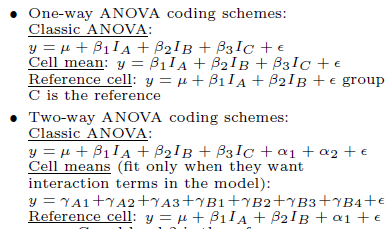
\includegraphics[scale=.6]{fig/an.png}\\
\textbf{Ref cell:} Group 1 is reference $\mu$ \ (grand mean)\\
\textbf{Cell mean:} all of the $\B$'s equal group means\\

\textbf{Topic 14: Logistic Regression}\\
$E(y)=p=\frac{\exp(\B_0+\B_1x)}{1+\exp(\B_0+\B_1x)}=\frac{1}{1+\exp(-\B_0-\B_1x)}$\\
$\frac{p}{1-p}=exp(\B_0+\B_1x)$\\
$logit(p_i)=\log\left(\frac{p_i}{1-p_i}\right)=\B_0+\B_1x+\dots$\\
$=\B_0+\B_1x_{i1}+\B_2x_{i2}+\dots+\B_{p-1}x_{i,p-1} \  (x\in 0,1)$\\ $OR=\frac{p_1/(1-p_1)}{p_2/(1-p_2)}=\frac{\exp(\B_0+\B_1(1))}{\exp(\B_0+\B_1(0))}=\exp(\B_0+\B_1(1)-\B_0-\B_1(0))=\exp(\B_1)$ \ $\log(OR)=\B_1$\\
95\% CI OR $(\log(OR)=\hat{\B_1})$ $\exp(\hat{\B_1}\pm 1.96se)$\\
$y_i\sim Bern(p_i) \ i=1,\dots,n$ ys ind of each other\\
LRT whether $k_{th}$ covariate affects $P(success)$ $H_0:\B_k=0$\\
Interaction $\ra$ LRT of full vs reduced\\
$H_0:$ interaction not significant\\
LRT comparing nested models: $-2\log(L(smaller))-(-2\log(L(larger)))$\\
$H_0\sim \chi^2_k \quad k=df_{larger}-df_{smaller}$
$H_0:\B_j=B_{jk(interaction)}=0$\\
$Var=p(1-p)$\\

\textbf{Topic 15: Mixed Effect Model}\\
everything is the same as for regression models\\ 
only difference is covariates\\
Y=fixed effects + random effects + error\\ 
$Y_i+X_i\B+Z_ib_i+\epsilon_i$\\
$Z_i$ indicator vars for cluster(family)membership\\
$b_i$ q-dim vector of random effects\\
\textbf{Blocking}:
group homogeneous exper units together to form
block, assign treats at random to exper units within block\\
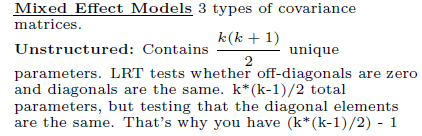
\includegraphics[scale=.6]{fig/not.png}\\
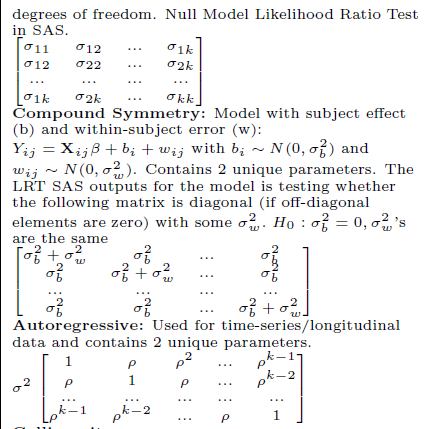
\includegraphics[scale=.6]{fig/notes.png}\\
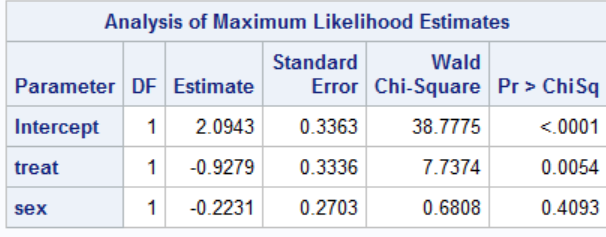
\includegraphics[scale=.6]{fig/me.png}\\
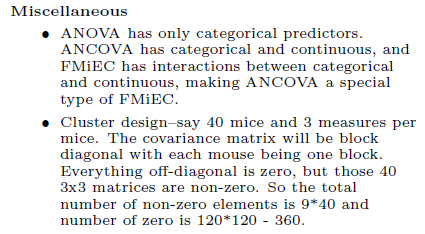
\includegraphics[scale=.6]{fig/misc.png}\\
\end{multicols*} 
\end{document}



